\begin{figure}[tbp]
\centering
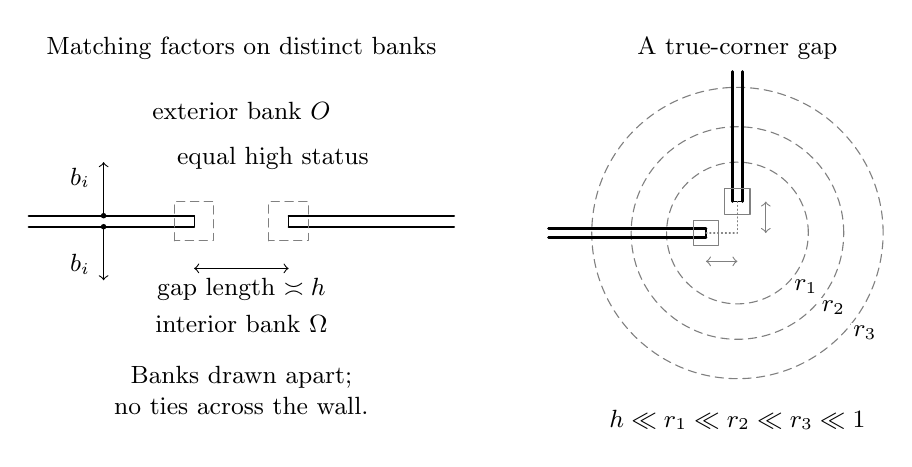
\begin{tikzpicture}[x=1cm,y=1cm,font=\small,line cap=round,line join=round]
  \node[align=center] at (2.7,4.5) {Matching factors on distinct banks};
  \node at (2.7,3.7) {exterior bank $O$};
  \node at (2.7,1.0) {interior bank $\Omega$};
  \foreach \y in {2.23,2.37} {
    \draw[line width=.8pt] (0,\y) -- (2.1,\y);
    \draw[line width=.8pt] (3.3,\y) -- (5.4,\y);
  }
  \draw (2.1,2.23) -- (2.1,2.37);
  \draw (3.3,2.23) -- (3.3,2.37);
  \draw[gray,densely dashed] (1.85,2.05) rectangle (2.35,2.55);
  \draw[gray,densely dashed] (3.05,2.05) rectangle (3.55,2.55);
  \fill (.95,2.37) circle (.035);
  \fill (.95,2.23) circle (.035);
  \draw[->] (.95,2.4) -- (.95,3.05);
  \draw[->] (.95,2.2) -- (.95,1.55);
  \node[left] at (.9,2.85) {$b_i$};
  \node[left] at (.9,1.75) {$b_i$};
  \node at (3.1,3.1) {equal high status};
  \draw[<->] (2.1,1.7) -- (3.3,1.7);
  \node[below] at (2.7,1.7) {gap length $\asymp h$};
  \node[align=center] at (2.7,.15)
    {Banks drawn apart;\\no ties across the wall.};
  \begin{scope}[shift={(9,2.15)}]
    \foreach \radius in {.9,1.35,1.85} {
      \draw[gray,densely dashed] (0,0) circle (\radius);
    }
    \draw[line width=1pt] (-2.4,.06) -- (-.4,.06);
    \draw[line width=1pt] (-2.4,-.06) -- (-.4,-.06);
    \draw[line width=1pt] (-.06,.4) -- (-.06,2.05);
    \draw[line width=1pt] (.06,.4) -- (.06,2.05);
    \draw (-.4,-.06) -- (-.4,.06);
    \draw (-.06,.4) -- (.06,.4);
    \draw[gray,densely dotted] (-.4,0) -- (0,0) -- (0,.4);
    \draw[gray] (-.56,-.16) rectangle (-.24,.16);
    \draw[gray] (-.16,.24) rectangle (.16,.56);
    \node[below right,fill=white,inner sep=1pt] at (.68,-.55) {$r_1$};
    \node[below right,fill=white,inner sep=1pt] at (1.03,-.82) {$r_2$};
    \node[below right,fill=white,inner sep=1pt] at (1.43,-1.14) {$r_3$};
    \draw[<->,gray] (-.4,-.36) -- (0,-.36);
    \draw[<->,gray] (.36,0) -- (.36,.4);
    \node[align=center] at (0,2.35) {A true-corner gap};
    \node[below] at (0,-2.12) {$h\ll r_1\ll r_2\ll r_3\ll1$};
  \end{scope}
\end{tikzpicture}
\caption{Paired walls and the local geometry of gap closure. Each surviving wall has distinct interior and exterior bank incidences, opposite wire designations, and matching factors $b_i$ evaluated with their own normals. Opening a straight gap produces two separately buffered tips; at a true corner, comparable lengths are removed on both incident sides. The dotted corner records where the filled wall would lie and supplies no connection or boundary segment for a Jordan closure. The nested radii satisfy $h\ll r_1\ll r_2\ll r_3\ll1$, with the mesh limit taken before gap closure. All geometry is schematic.}
\label{fig:paired-walls}
\end{figure}
